\documentclass[12pt,journal, a4paper]{IEEEtran}



\usepackage{graphicx}   % Written by David Carlisle and Sebastian Rahtz


\usepackage{url}        % Written by Donald Arseneau


\usepackage{amsmath}    % From the American Mathematical Society
                        % A popular package that provides many helpful c
\usepackage{listings}

\usepackage{caption}

\usepackage{float}

% Your document starts here!
\begin{document}

% Define document title and author
    \title{CS 553: Cloud Computing\\Understanding the cost of the cloud}
    \author{Thomas Dubucq / Tony Forlini / Virgile Landeiro Dos Reis
    \thanks{Advisor: Ioan Raicu, IIT 2014/2015.}}
    \markboth{Illinois Institute Of Technology}{}
    \maketitle

% Write abstract here
\begin{abstract}
The main purpose of this project is to grasp the importance of economic concerns regarding cloud computing. Since cloud computing becomes widespread within the industry of computer science, the management of prices has become a huge topic of cloud computing these years. We are to study the incentives of setting up a public rather than a private cloud. 
\end{abstract}

% Each section begins with a \section{title} command
\section{Introduction}
We are to compare the price of setting up a public cloud using Amazon Web Services, and the price of buying all the ressources in order to build a private cloud. In our study, we will consider different cloud size expressed in Flops, (floating point operations per second). Finally we will see in what extent it is interesting to use public ressources rather than buying and setting up a private cloud from scratch. 
% Main Part
\section{Cost of Amazon instances}
In this section we will study the cost a compute cloud according to the amount of floating operations per seconds they provide. We will make the assumption that one EC2 instance provides 4.4 GFlops and compute the cost of the compute cloud for every following type a Amazon instance: t2.small, m3.large, c3.8xlarge, g2.2xlarge, r3.4xlarge, i2.8xlarge, and hs1.8xlarge. Since those instances don't provide the same kind of compute (some are GPU intensive, other are memory or disk intensive) we need to take in account the ammount of Flops provided by each instance. Our graph will plot the subsequent price from a cloud providing from 1 GFlop to 1PFlop. We first need to determine the GFlop provided by every instance and then compute the price per hour per flop. We get the following array:\\
\begin{table}[H]
\begin{center}

   \begin{tabular}{ | c | c | }

     \hline

     Instance type & Hourly Price/GFlop  \\ \hline

     t2.small & \$0.0059\\ \hline

     m3.large & \$0.0049\\ \hline

     c3.8xlarge & \$0.0035\\ \hline

     g2.2xlarge & \$0.0056\\ \hline
     
     r3.4xlarge & \$0.0061\\ \hline
     
     i2.8xlarge & \$0.014\\ \hline

     hs1.8xlarge & \$0.029\\

     \hline
        
   \end{tabular}
 \end{center} 
\end{table}
Note that we made an approximation while computing the hourly price per instance, given that for a small ammount of Flops, we might not need more instances to increase the ammount of Flop. Then the price per Flop becomes greater because we cannot rent "small parts" of instances.  
Now we are able to compute the hourly price per instance type using the hourly pricing from Amazon instances and we plot it on the following graph:\\
 

\begin{figure}[H]
\centering
\captionsetup{justification=centering}
\begin{tabular}{cc}
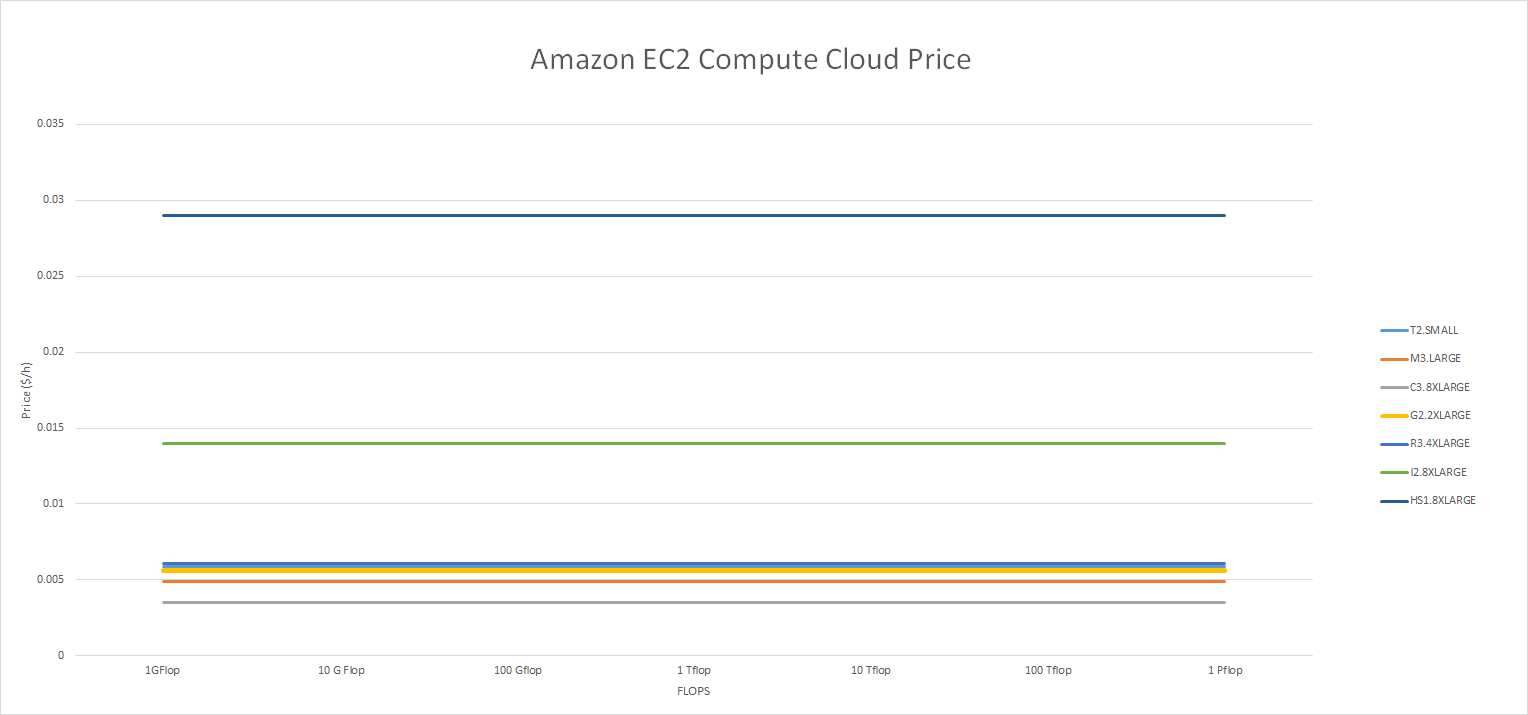
\includegraphics[width=9cm, height=5cm]{Cloud_Amazon_price.png}
\end{tabular}
\caption{Public Cloud price}
\end{figure}

Unlike what we could expect from the Amazon hourly pricing per instance, the small instances are not the cheapest as we increase the computation need for our cloud. Then we require a large number of small instances to reach our needs in term of Flops, which is more expensive than using instances with more computational power such as GPU instances. On the other hand, instances such as hs1.8xlarge and i2.8xlarge are very expensive and are most likely to be used by a small number of users. Still, the fact that Amazon provides such powerful instances can lead users to consume other cheaper Amazon's products and the ammount of such powerful instances owned by Amazon must be wisely chosen. 
 

   
\section{Cost of a private cloud}

In this section we will compute the cost of buying and setting up a private cloud of which instances are built similarly to Amazon's instances. That means that we will compute the price of each equivalent instance and consider a 5 year usage. Then we will factorize some components of each instances such as CPUs or racks to share them across different machines.\\

We will also take in account the price of the power supply, the cooliing price and the administration cost for our private cloud, which is a very important part of the budget. For instance for low Flops ammount, the administration cost will be important beacause one person will be paid to monitor one instance, but by increasing Flops, this cost will drop until more administrators are required.\\

To find the equivalents to every Amazon instance type, we looked for equivalent new hardware with a price as low as possible. To compute the equivalent CPU price, we looked for the number of ECU (EC2 compute unit) and we chose the corresponding Intel CPU for each instance.
First we compute the private equivalent to every single Amazon instance in the table below:\\

\begin{table}[H]
\begin{center}

   \begin{tabular}{ | c | c | c | c | c | c | c | c | c |}

     \hline

     Component & t2.small & m3.large & c3.8xlarge & g2.2xlarge & r3.4xlarge & i2.8xlarge & hs1.8xlarge  \\ \hline \hline

     CPU & \$1,329 & \$1,329 & \$1,727 & \$1,600 & \$939 & \$1,846 & \$939 \\ \hline 

     Memory & \$288  & \$576 & \$628 &\$82 & \$192 & \$3,328 & \$ 1,440\\ \hline


     Rack*  & \$1,126.00 & \$1,126.00 & \$383 & \$383 & \$1,126.00 & \$1,126.00 &\\ \hline
     
     Disk & X & \$94 & \$529 & \$48 & \$290 & \$94 & \$800\\ \hline
     
     GPU & X & X & X & \$90 & X & X & X\\ \hline \hline

     Total/unit & \$2,743.00(12instances) & \$3,126.00(6instances) & \$3,267 & \$2,502 & \$2,547.49 & \$6,394.99 & \$4,305.00\\ \hline 
     
    Total/instance & \$228.58 & \$521.00 & \$3,267 & \$2,502 & \$2,547.49 & \$6,394.99 & \$4,305.00\\ \hline
        \end{tabular}
 \end{center} 
\end{table}

$Rack* = motherboard, network,alimentation,case$ 
\begin{table}[H]
\begin{center}

   \begin{tabular}{ | c | c | c |}

     \hline

     Cooling & 1medium AC window unit per rack & power cumsumption 0.9 kw \\ \hline
     
     Power & \$0.10/kWh &  \\ \hline
     
     Administration &  1 administrator for 1000 units &  \$21/hour\\ \hline

     \hline
        
   \end{tabular}
 \end{center} 
\end{table}



Thus the main difference with the public cloud is that we have a fixed cost per instance per hour but we can factorize the administration, cooling and power price among instance although Amazon cannot do that with its pay as you go policy which has fixed prices for instances. We plot the comparison between the public and private clouds below.\\


As we forecasted, low scales involves a waste of administration ressources which is high for only few instances monitoring. We also see that our private instances have roughly the same price since the administration cost per hour and per flop is higher than the hardware or power cost per flop per hour. Then the price eventually remains steady for large scales.\\


Now we finally want to know which of the public or the private cloud is the most interesting and cheap. Thus we plot the the needed utilization of the private cloud from 1GFlop to 1PFlop for the different instance types in order to break even cost wise. For each instance, the percentage of utilization required to discount over the public cloud is plot acording to the scale of the cloud. If no value appears for low scale, it means that the public cloud is more profitable than the private one:

\newpage

\begin{figure}[H]
\centering
\captionsetup{justification=centering}
\begin{tabular}{cc}
\includegraphics[width=18cm, height=10cm]{g2989.png}
\end{tabular}
\caption{Public vs. private cloud}
\end{figure}
 

\begin{figure}[h!]
\centering
\captionsetup{justification=centering}
\begin{tabular}{cc}
\includegraphics[width=18cm, height=10cm]{bitmap.png}
\end{tabular}
\caption{Cost-wise breakpoint}
\end{figure}

\newpage
.\newpage
% Now we need a bibliography:
Finally, We see on figure 3 that for low scale clouds, it is more interesting to use a public cloud rather than buying everything and pay a huge price for administration which is not efficient for a five years utilization. However, when the cloud's scale increases to 10 TFlop the price of a private cloud becomes more profitable than which of the public because we amortize the administration cost increasing the scale of the cloud. This break-even points tend to converge with the ammount of Flops since the public cloud price remains constant.

\section{Conclusion}
To conclude, this project allowed us the understand the insight of how to buld a cloud by taking care of the economies of scale. Though our model was simplified in a certain extent by lack of detailed pricing and for the sake of clarity (we could have computed the cost of internet access, the buliding cost, the annex employees, the construction field etc...) it still gives us a good idea of what a private cloud could be and a comparison with the already existing and successful public clouds such as Amazon web services. \\

In a nutshell we can say that for small businesses such as startups renting a public cloud rather than buying is less expensive and thus more efficient. On the other hand we reach the break-even cost for a private cloud after having a cloud with about a dozen of TFlop. This profitablity then increases and converge with the scale of the cloud. This option is more adapted to big companies which furthermore won't have to worry about common issues such as security and geographic repartition of data for the sake of data integrity. 
\begin{thebibliography}{5}

    %Each item starts with a \bibitem{reference} command and the details thereafter.
    \bibitem{HOP96} % Transaction paper
http://aws.amazon.com/ec2/instance-types/
\bibitem{HOP96} 
http://aws.amazon.com/ec2/pricing/
\bibitem{HOP96} 
http://www.newegg.com/
\bibitem{HOP96} 
http://datasys.cs.iit.edu/projects/CloudStorage\_summary12.pdf.
\bibitem{HOP96} 
http://www.npr.org/blogs/money/2011/10/27/141766341/the-price-of-electricity-in-your-state
\bibitem{HOP96}
http://www.payscale.com/research/US/Job=Data\_Center\_Technician/Hourly\_Rate
\bibitem{HOP96} 
http://powersurvival.com/info.htm
\bibitem{HOP96} 
http://extreme.outervision.com/psucalculatorlite.jsp
\bibitem{HOP96}
http://www.supermicro.com/products/system/4U/7048/SYS-7048A-T.cfm
\bibitem{HOP96} 
http://www.kernelsoftware.com/products/catalog/supermicro.html
\end{thebibliography}

% Your document ends here!
\end{document}